% 1987 年上海卷第二题：y=x^(2/3) 的四个图象选项
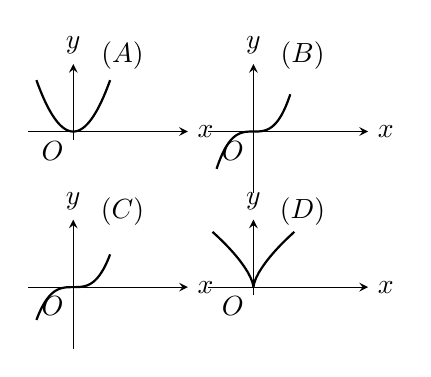
\begin{tikzpicture}[scale=0.52,>=stealth]
  \node at (1.2,1.85) {$(A)$};
  \draw[->] (-1.1,0)--(2.8,0) node[right] {$x$};
  \draw[->] (0,-0.2)--(0,1.65) node[above] {$y$};
  \draw[thick,domain=-0.9:0.9,samples=80] plot (\x,{1.55*\x*\x});
  \node[below left] at (0,0) {$O$};

  \begin{scope}[xshift=4.4cm]
    \node at (1.2,1.85) {$(B)$};
    \draw[->] (-1.1,0)--(2.8,0) node[right] {$x$};
    \draw[->] (0,-1.5)--(0,1.65) node[above] {$y$};
    \draw[thick,domain=-0.9:0.9,samples=80] plot (\x,{1.25*\x*\x*\x});
    \node[below left] at (0,0) {$O$};
  \end{scope}

  \begin{scope}[yshift=-3.8cm]
    \node at (1.2,1.85) {$(C)$};
    \draw[->] (-1.1,0)--(2.8,0) node[right] {$x$};
    \draw[->] (0,-1.5)--(0,1.65) node[above] {$y$};
    \draw[thick,domain=-0.9:0.9,samples=80] plot (\x,{1.1*\x*\x*\x});
    \node[below left] at (0,0) {$O$};
  \end{scope}

  \begin{scope}[xshift=4.4cm,yshift=-3.8cm]
    \node at (1.2,1.85) {$(D)$};
    \draw[->] (-1.1,0)--(2.8,0) node[right] {$x$};
    \draw[->] (0,-0.2)--(0,1.65) node[above] {$y$};
    \draw[thick,domain=-1.0:0,samples=80] plot (\x,{1.35*abs(\x)^(2/3)});
    \draw[thick,domain=0:1.0,samples=80] plot (\x,{1.35*abs(\x)^(2/3)});
    \node[below left] at (0,0) {$O$};
  \end{scope}
\end{tikzpicture}
